%%
%% This is file `sample-sigconf.tex',
%% generated with the docstrip utility.
%%
%% The original source files were:
%%
%% samples.dtx  (with options: `sigconf')
%%
%% IMPORTANT NOTICE:
%%
%% For the copyright see the source file.
%%
%% Any modified versions of this file must be renamed
%% with new filenames distinct from sample-sigconf.tex.
%%
%% For distribution of the original source see the terms
%% for copying and modification in the file samples.dtx.
%%
%% This generated file may be distributed as long as the
%% original source files, as listed above, are part of the
%% same distribution. (The sources need not necessarily be
%% in the same archive or directory.)
%%
%% The first command in your LaTeX source must be the \documentclass command.
\documentclass[sigconf,noacm]{acmart}
\settopmatter{printacmref=false} % Removes citation information below abstract
\renewcommand\footnotetextcopyrightpermission[1]{} % removes footnote with conference information in first column
\pagestyle{plain} % removes running headers
\usepackage{subcaption}
\usepackage{minted}

%%
%% \BibTeX command to typeset BibTeX logo in the docs
\AtBeginDocument{%
  \providecommand\BibTeX{{%
    \normalfont B\kern-0.5em{\scshape i\kern-0.25em b}\kern-0.8em\TeX}}}

%% Rights management information.  This information is sent to you
%% when you complete the rights form.  These commands have SAMPLE
%% values in them; it is your responsibility as an author to replace
%% the commands and values with those provided to you when you
%% complete the rights form.
\setcopyright{acmcopyright}
\copyrightyear{2018}
\acmYear{2018}
\acmDOI{10.1145/1122445.1122456}

%% These commands are for a PROCEEDINGS abstract or paper.
\acmConference[CS294 Project]{Building an RTL Coverage Proxy Model for RISC-V CPUs}
{}{}

\tolerance=1
\emergencystretch=\maxdimen
\hyphenpenalty=10000
\hbadness=10000

\begin{document}

\title{Building an RTL Coverage Proxy Model for RISC-V CPUs}

\author{Vighnesh Iyer}
\email{vighnesh.iyer@berkeley.edu}
\affiliation{%
\institution{UC Berkeley}}
  %\institution{The Th{\o}rv{\"a}ld Group}
  %\streetaddress{1 Th{\o}rv{\"a}ld Circle}
  %\city{Hekla}
  %\country{Iceland}}

\renewcommand{\shortauthors}{Vighnesh Iyer}

\begin{abstract}
RTL verification consumes the majority of time in the hardware design cycle, so there is interest in increasing the efficiency of existing dynamic verification methods.
Typical dynamic verification loops utilize a constrained random stimulus generator to drive a design-under-test, while checking for buggy states and trajectories, and collecting RTL coverage data.
It is usually impossible to exclude the possiblity of bugs altogether, so verification engineers focus on maximizing RTL coverage as a proxy for the thoroughness of their testing efforts.

We propose the design of an RTL coverage proxy model which aims to predict structural RTL coverage from pre-RTL-simulation features.
Such a model can be used to: 1) avoid the wasteful RTL simulation of redundant or inferior tests, 2) provide DV engineers with insights on correlations between their stimulus generator and coverage to help with constraint and bias tuning, and 3) make automatic random variable distribution tuning viable by bypassing slow RTL simulation.


%During the design process, a considerable amount of data is produced such as per-test RTL coverage from nightly random regressions.
%Those same tests are executed on fast functional models which also produce large amounts of data such as C++ coverage, logs, and transaction and execution traces.

%We propose the construction of an RTL coverage prediction model which can estimate RTL coverage from functional simulation, to direct test selection and hit coverage goals faster.

%During unit design, nightly random regressions provide considerable per-test coverage data.
%Closing coverage by running regression workloads and random stimulus takes a long time and must be repeated if the RTL were to change.

%Ideally one only needs to simulate the specific stimulus vectors that would be likely to hit any uncovered coverpoints.
%However, to determine the RTL coverage of any proposed test stimulus requires slow RTL simulation or human intuition.
\end{abstract}

\maketitle

\section{Background}

\subsection{Digital Hardware Design}

The vast majority of digital systems are built using synchronous digital circuits.
These circuits can be described with a simple abstraction, consisting of 1) state and 2) update rules.
The state of a digital circuit is just `a bunch of bitvectors' and the update rules specify how every state bitvector should be updated as a logic function of all the state bitvectors.
The state is updated according to the update rules on the rising ($0 \rightarrow 1$) edge of a special one-bit \textit{clock} signal, which continuously toggles from $0 \rightarrow 1 \rightarrow 0$ at a fixed frequency.

Of course, digital circuits are usually not closed systems, otherwise there would be no way to pass data into them or get data out.
In addition to state and update rules, digital circuits also have top-level (primary) inputs and outputs, which are also bitvectors.
The update rules are now functions of both the current state and the primary inputs.
The primary outputs are a function of the current state and the primary inputs in the most general case (allowing combinational coupling of primary inputs to outputs).

\subsubsection{Transition System Representation}
We can formally represent a synchronous digital circuit as a transition system $T$.

\begin{equation*}
  T = (S, I, PI, R, PO)
\end{equation*}

where,

\begin{itemize}
  \item $S = $ a set of state elements (bitvectors)
  \item $I = $ a set of initial state assignments
  \item $PI = $ a list of the top-level (primary) inputs (bitvectors) to the circuit
  \item $R = $ the transition relation or update rules $R: S \times PI \rightarrow S$
  \item $PO = $ a list of the top-level (primary) outputs (bitvectors) of the circuit and their update rule $PO: S \times PI$
\end{itemize}

\subsubsection{Hardware Design Languages}

Synchronous digital circuits can be described in several different hardware design languages (HDLs) that operate at different levels of abstraction (all the way from software-like algorithmic/imperative descriptions of desired circuit behavior, down to transistor-level netlists).
The HDL abstraction level that matches the transition system representation of a circuit is called register-transfer level (RTL).
The primitives in an RTL-level HDL are state elements, update rules, and ports, and these can be desugared to transition systems.

The vast majority of digital circuits are written at the RTL-level since it gives the designer precise control over the state and logic that will end up on the chip.
The most popular RTL-level HDL is Verilog (which can also represent lower levels of circuit abstraction such as gate-level or transistor-level).
Here is an example of Verilog code:

\begin{minted}{verilog}
module alu(input [7:0] a, b,
           input op, clk, output reg [8:0] o);
  always_ff @(posedge clk)
    if (op) o <= a + b;
    else    o <= a - b;
endmodule
\end{minted}

This describes a transition system with one state element \texttt{o}, a single update rule \texttt{o <= op ? (a+b) : (a-b)}, three primary inputs \texttt{(a, b, op)}, and one primary output \texttt{o} (which is driven directly by the state element).

\subsection{Digital Hardware Simulation}

Simulating a synchronous digital circuit is equivalent to simulating its underlying transition system.
Verilog simulators implement a function $s$:

\begin{equation*}
  s(T, PI_0, PI_1, \dots, PI_n) = (PO_0, PO_1, \dots PO_n)
\end{equation*}

where given a concrete binding of each primary input for $n$ clock cycles of simulation, the simulator will return a sequence of concrete bindings of each primary output.

In practice, RTL testbenches invoke the underlying simulator one clock cycle at a time, by providing primary inputs for one cycle, telling the simulator to execute the update rules, inspecting the primary outputs, and repeating this process.
A popular Verilog simulator that supports this mode of execution is Verilator, and we use it for our benchmarks.

\subsection{Digital Hardware Verification}

\begin{figure}
  %\centering
  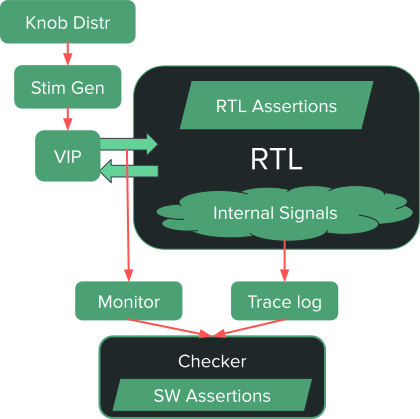
\includegraphics[width=0.65\linewidth]{figs/dynamic_verif.pdf}
  \caption{A typical dynamic verification environment}
  \label{fig:dynamic_verif}
\end{figure}

Merely simulating a transition system by providing it with inputs doesn`t tell us if anything has gone wrong, since the simulation behavior is always well defined.
This is in contrast to user-space software which has `universal' modes of failure such as segfaults or stack overflows, which are failures that exist independently of the application logic itself.

In hardware verification, bugs are detected by assertions baked into the Verilog RTL or by 


\bibliographystyle{ACM-Reference-Format}
\bibliography{references}

\appendix

\end{document}
\endinput
